\section{Μηχανή Αναζήτησης}
Ο Χρήστης στην κορυφή της ιστοσελίδας θα βρει μια μπάρα αναζήτησης που του επιτρέπει να ψάξει άτομα, εταιρίες, χώρες και είδη ταινιών. Σε κάθε γράμμα που θα πληκτρολογήσει θα του εμφανίζονται ανάλογα αποτελέσματα για να επιλέξει. Ένα αποτέλεσμα αποτελείται από μια φωτογραφία και έναν όνομα. Για παράδειγμα αν το αποτέλεσμα είναι μια χώρα η εικόνα θα είναι η σημαία της χώρας και το όνομα, το όνομα της. Αν το αποτέλεσμα είναι ένα άτομο η εικόνα θα είναι μια φωτογραφία του ατόμου, αν υπάρχει αλλιώς μια προκαθορισμένη φωτογραφία, και το όνομα του. Αν είναι είδος ταινίας θα υπάρχει ένα εικονίδιο για εικόνα και το όνομα του είδους. Και αν είναι εταιρία το λογότυπο της εταιρίας, αν υπάρχει αλλιώς ένα προκαθορισμένο εικονίδιο κτηρίου όπως φαίνεται στην εικόνα \ref{demo:searchbar} στο 2ο αποτέλεσμα των εταιριών, και το όνομα της. Ο Χρήστης πρέπει να επιλέξει ένα από τα προτεινόμενα αποτελέσματα καθώς η γενική αναζήτησης με το πλήκτρο "Enter" δεν υποστηρίζεται.

\begin{figure}[H]
  \centering
  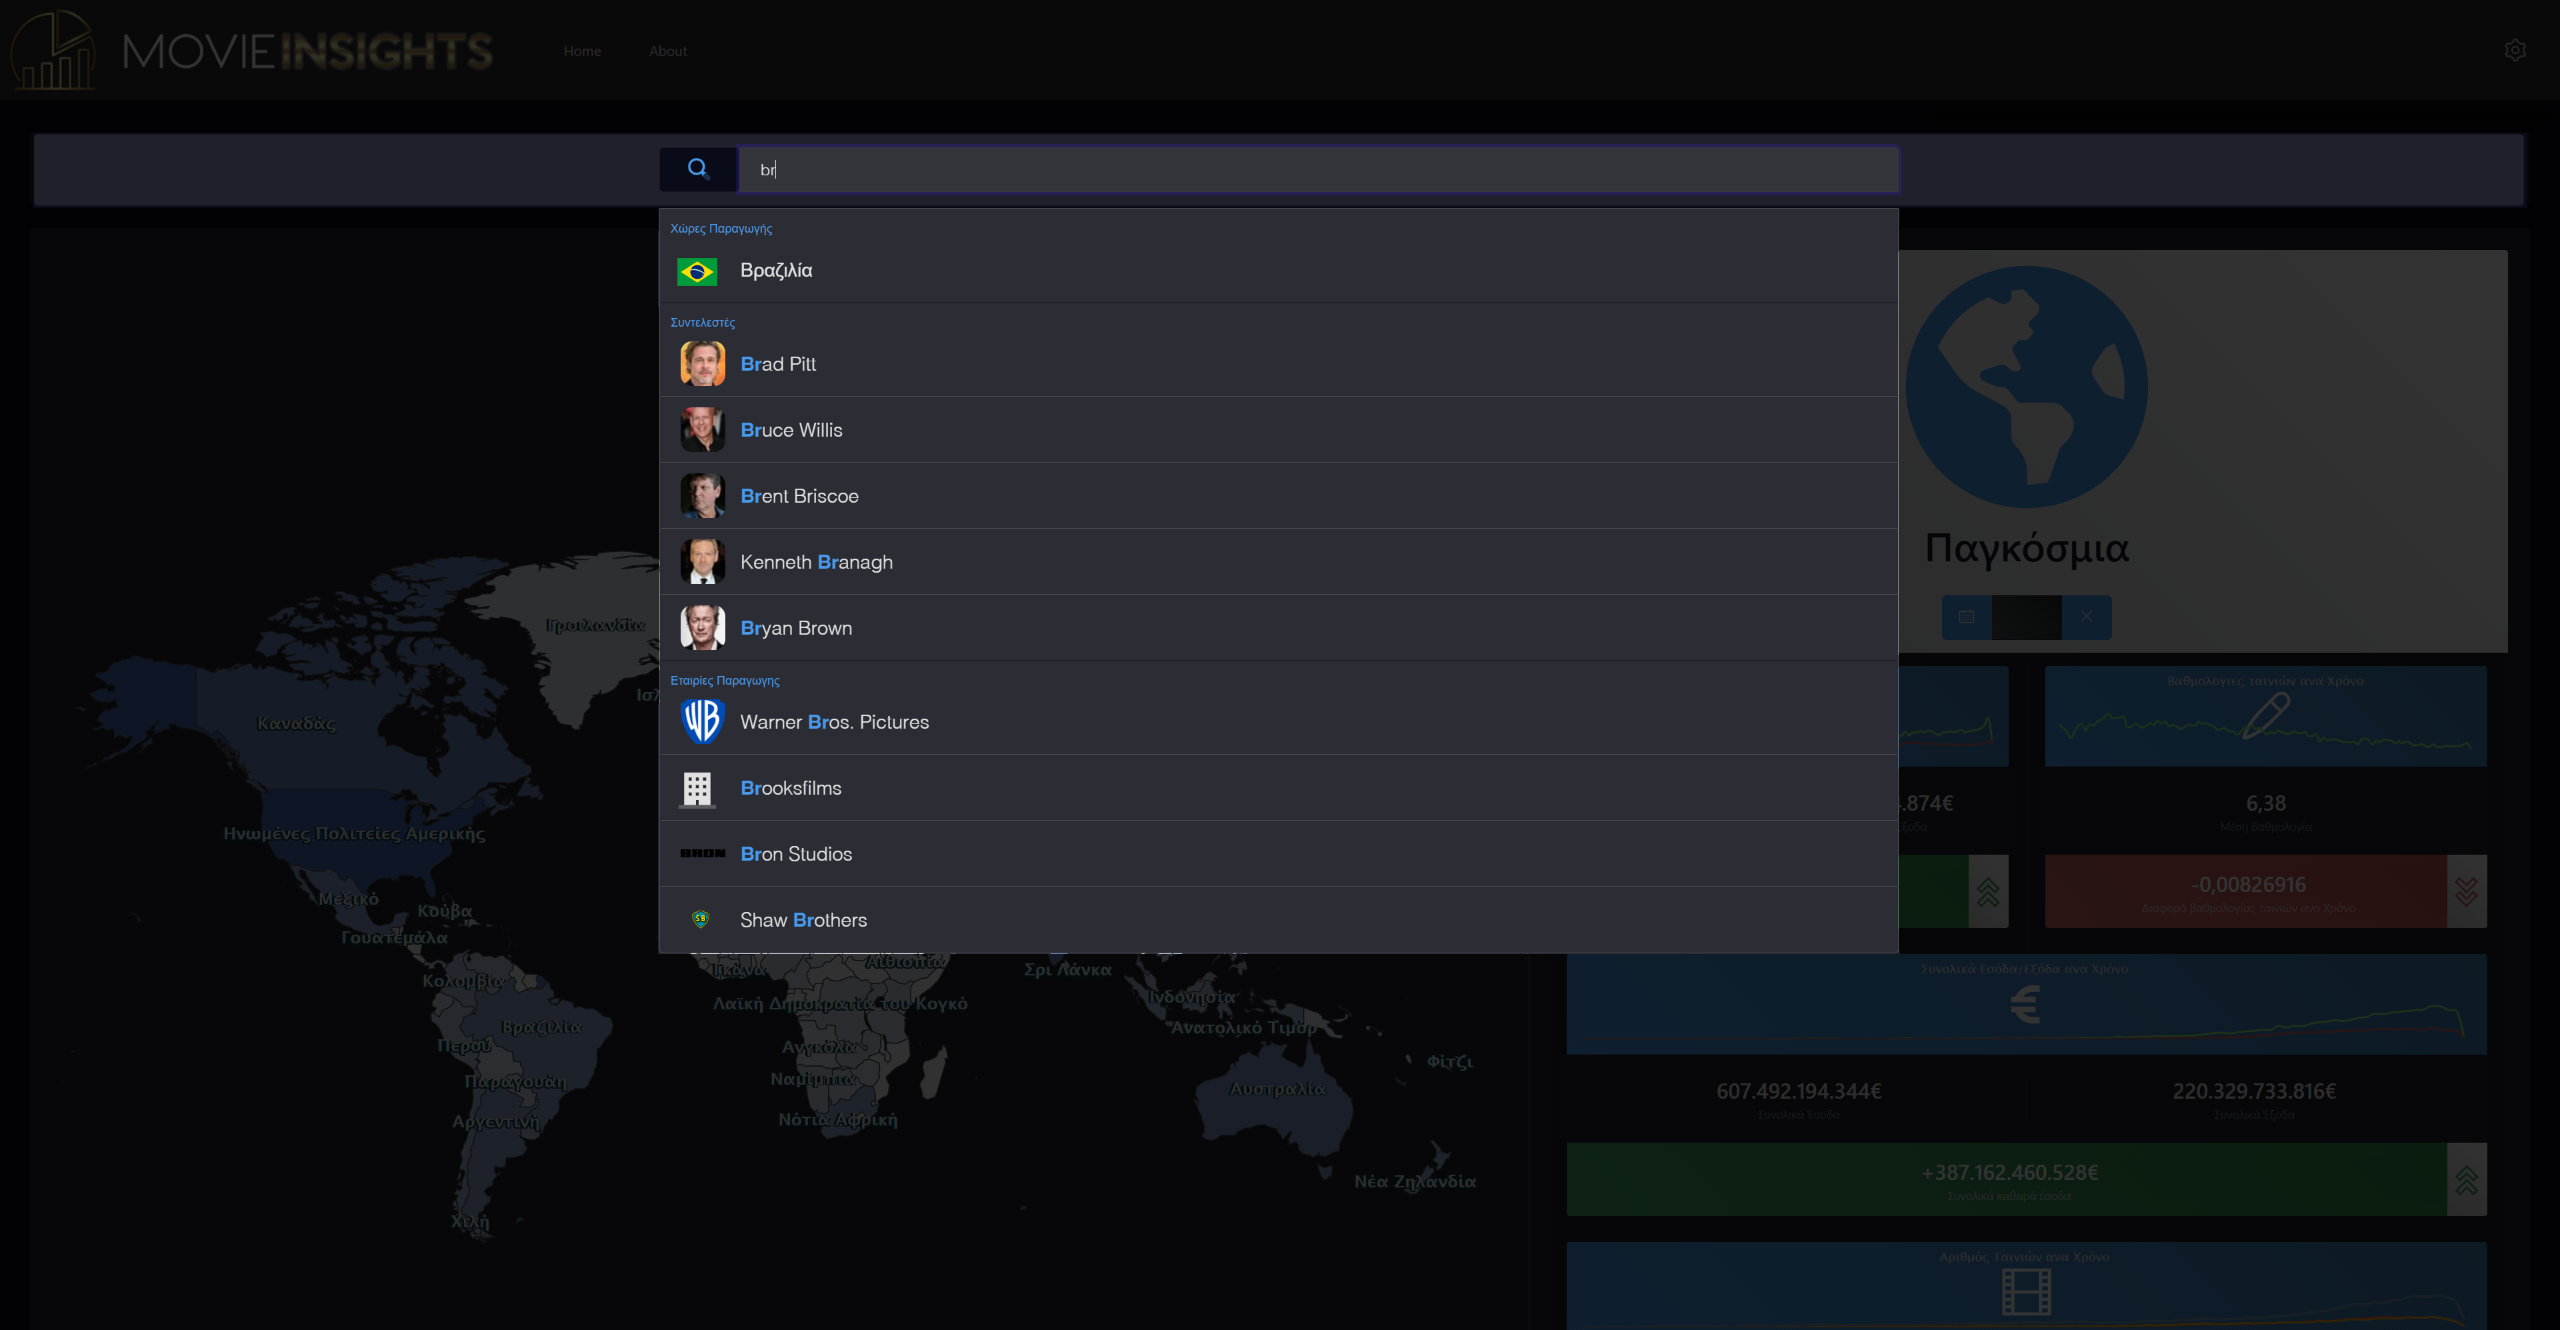
\includegraphics[width=145mm]{Chapters/6 - Manual/Images/main_page_searchbar.png}
  \caption{Γραμμή Αναζήτησης}
  \label{demo:searchbar}
\end{figure}